\section{Results}
\label{sec:results}
%Explain factually what you found... leave interpretation of what it means for the final discussion section. Here you would include plots of what you found or comparison tables.

\subsection{Improvised force plate kymograph}
Heel versus toe-strike two trials. Toe-strike only shows lateral movement of rig, primarily with left foot. 
\begin{figure}
\begin{center}
a \includegraphics[width=0.29\columnwidth]{figures/results3.png}
b 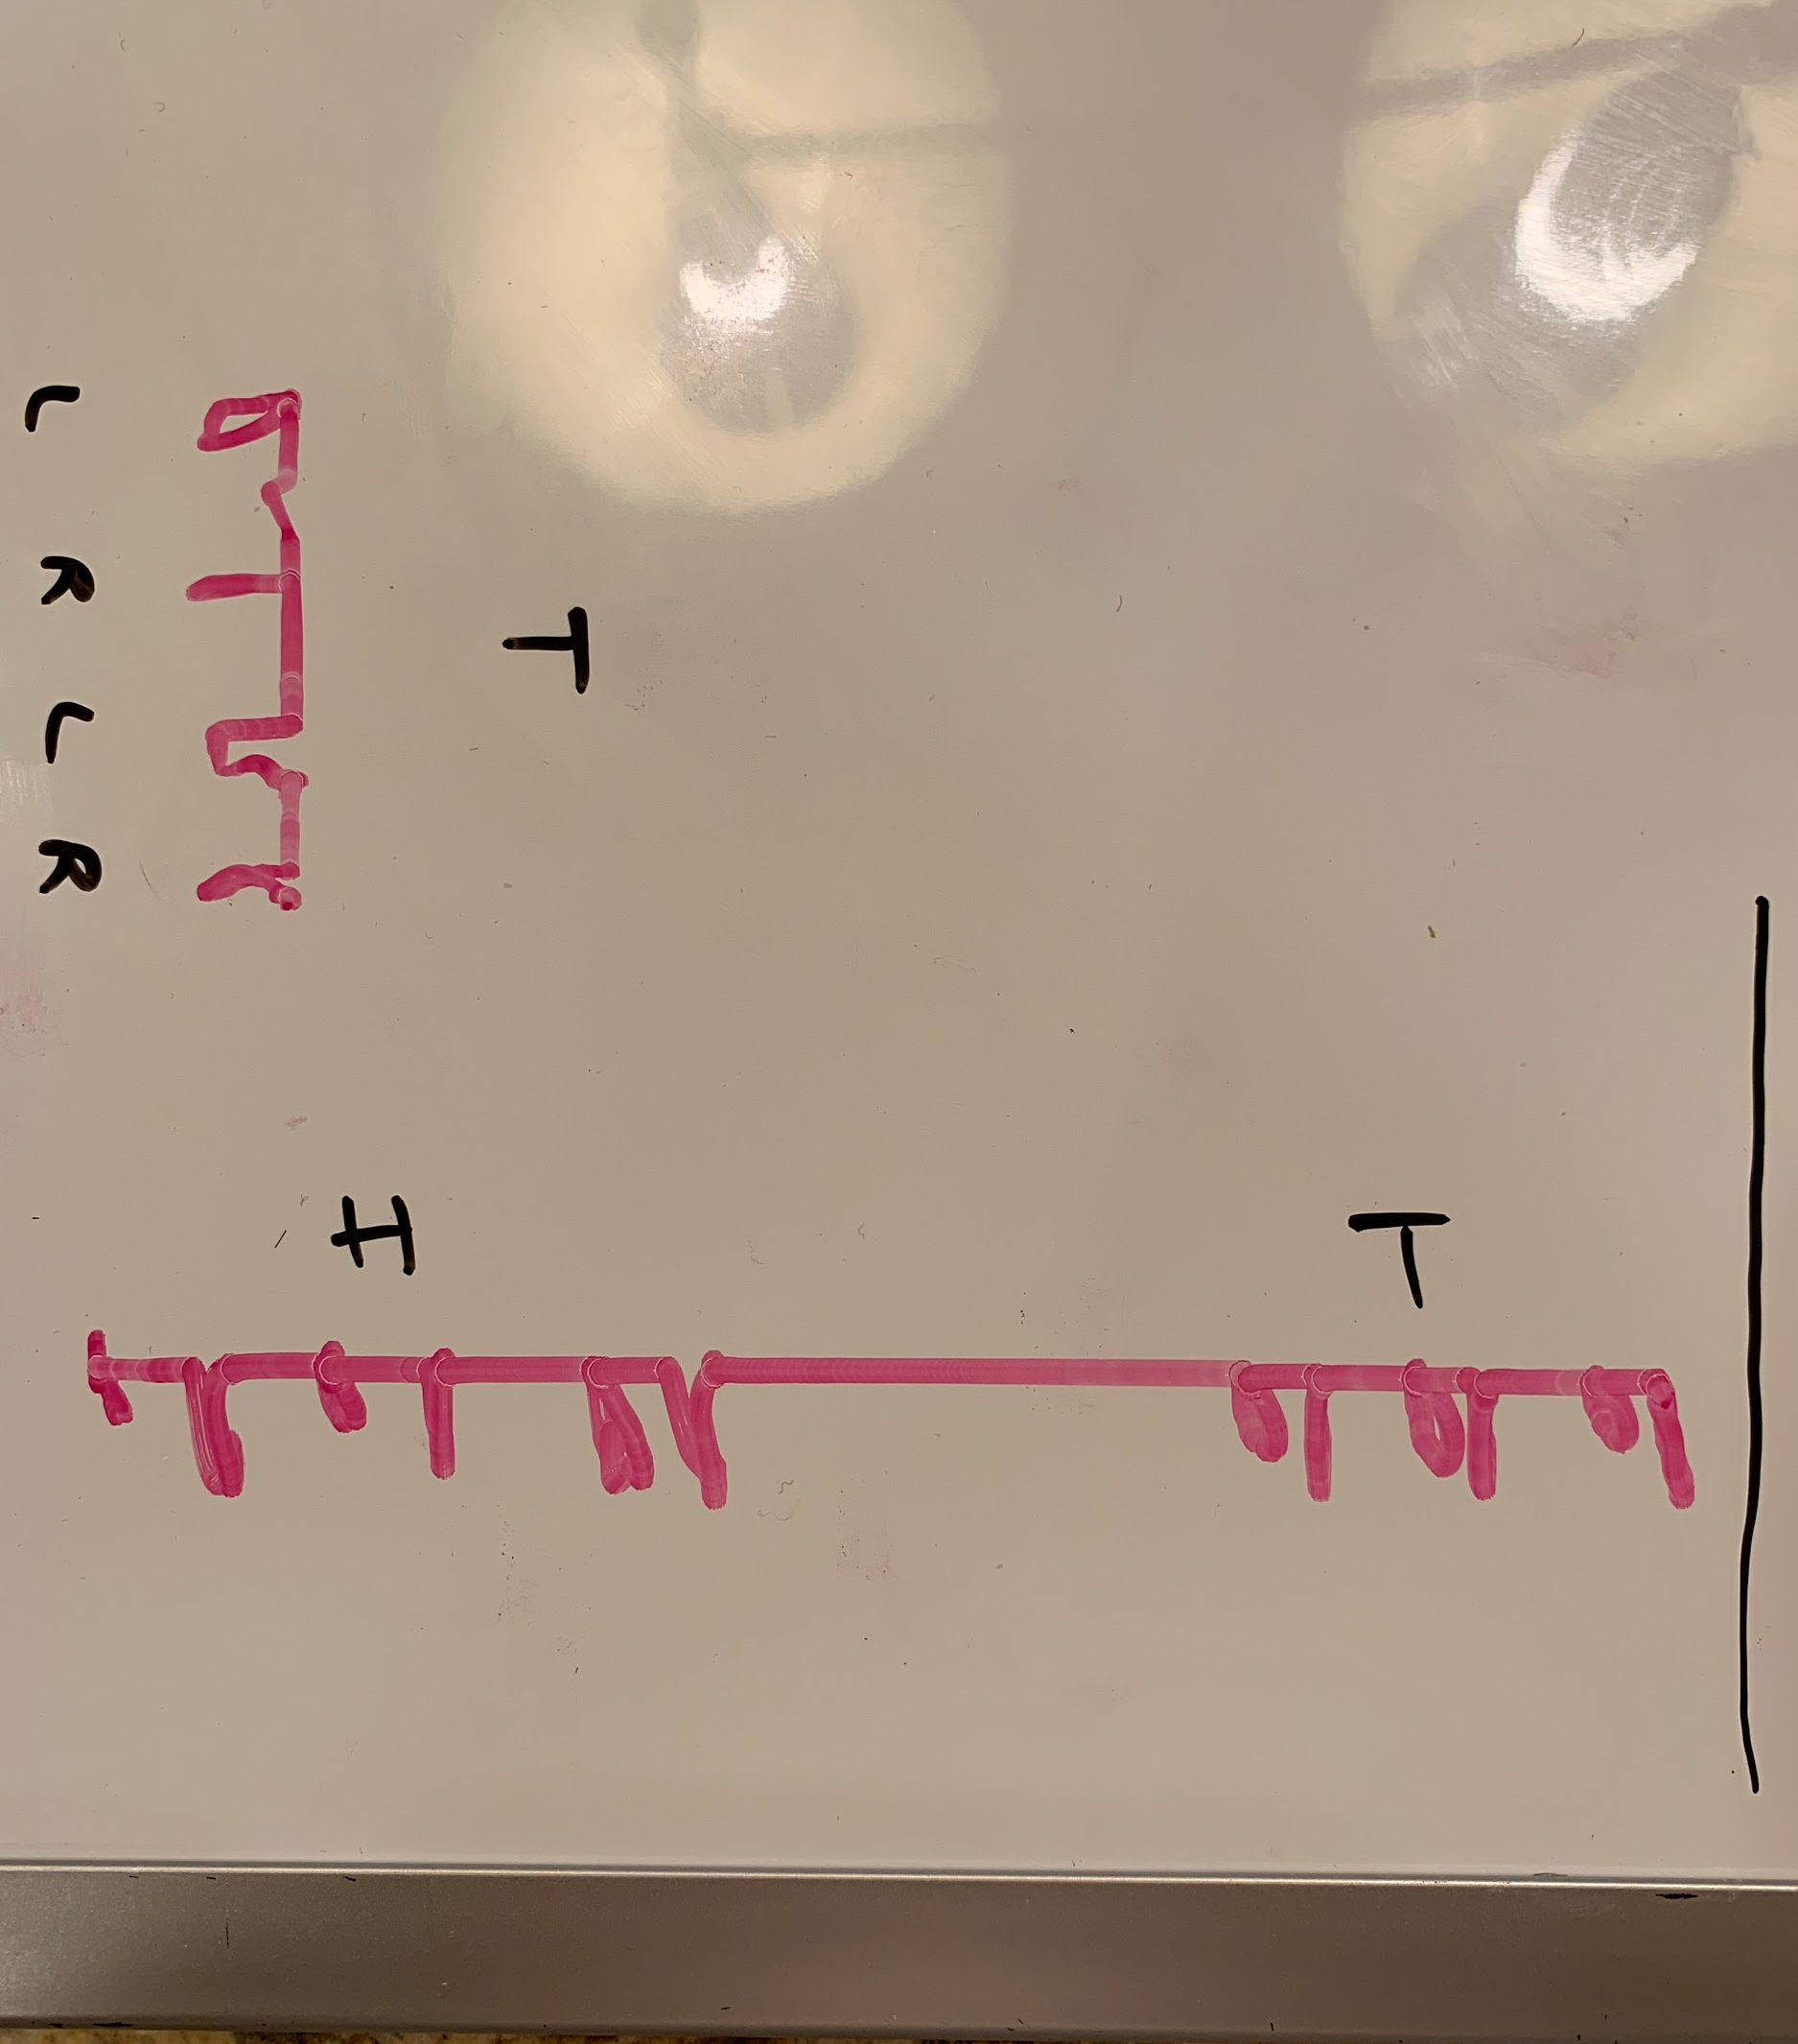
\includegraphics[width=0.29\columnwidth]{figures/results4.png}
c 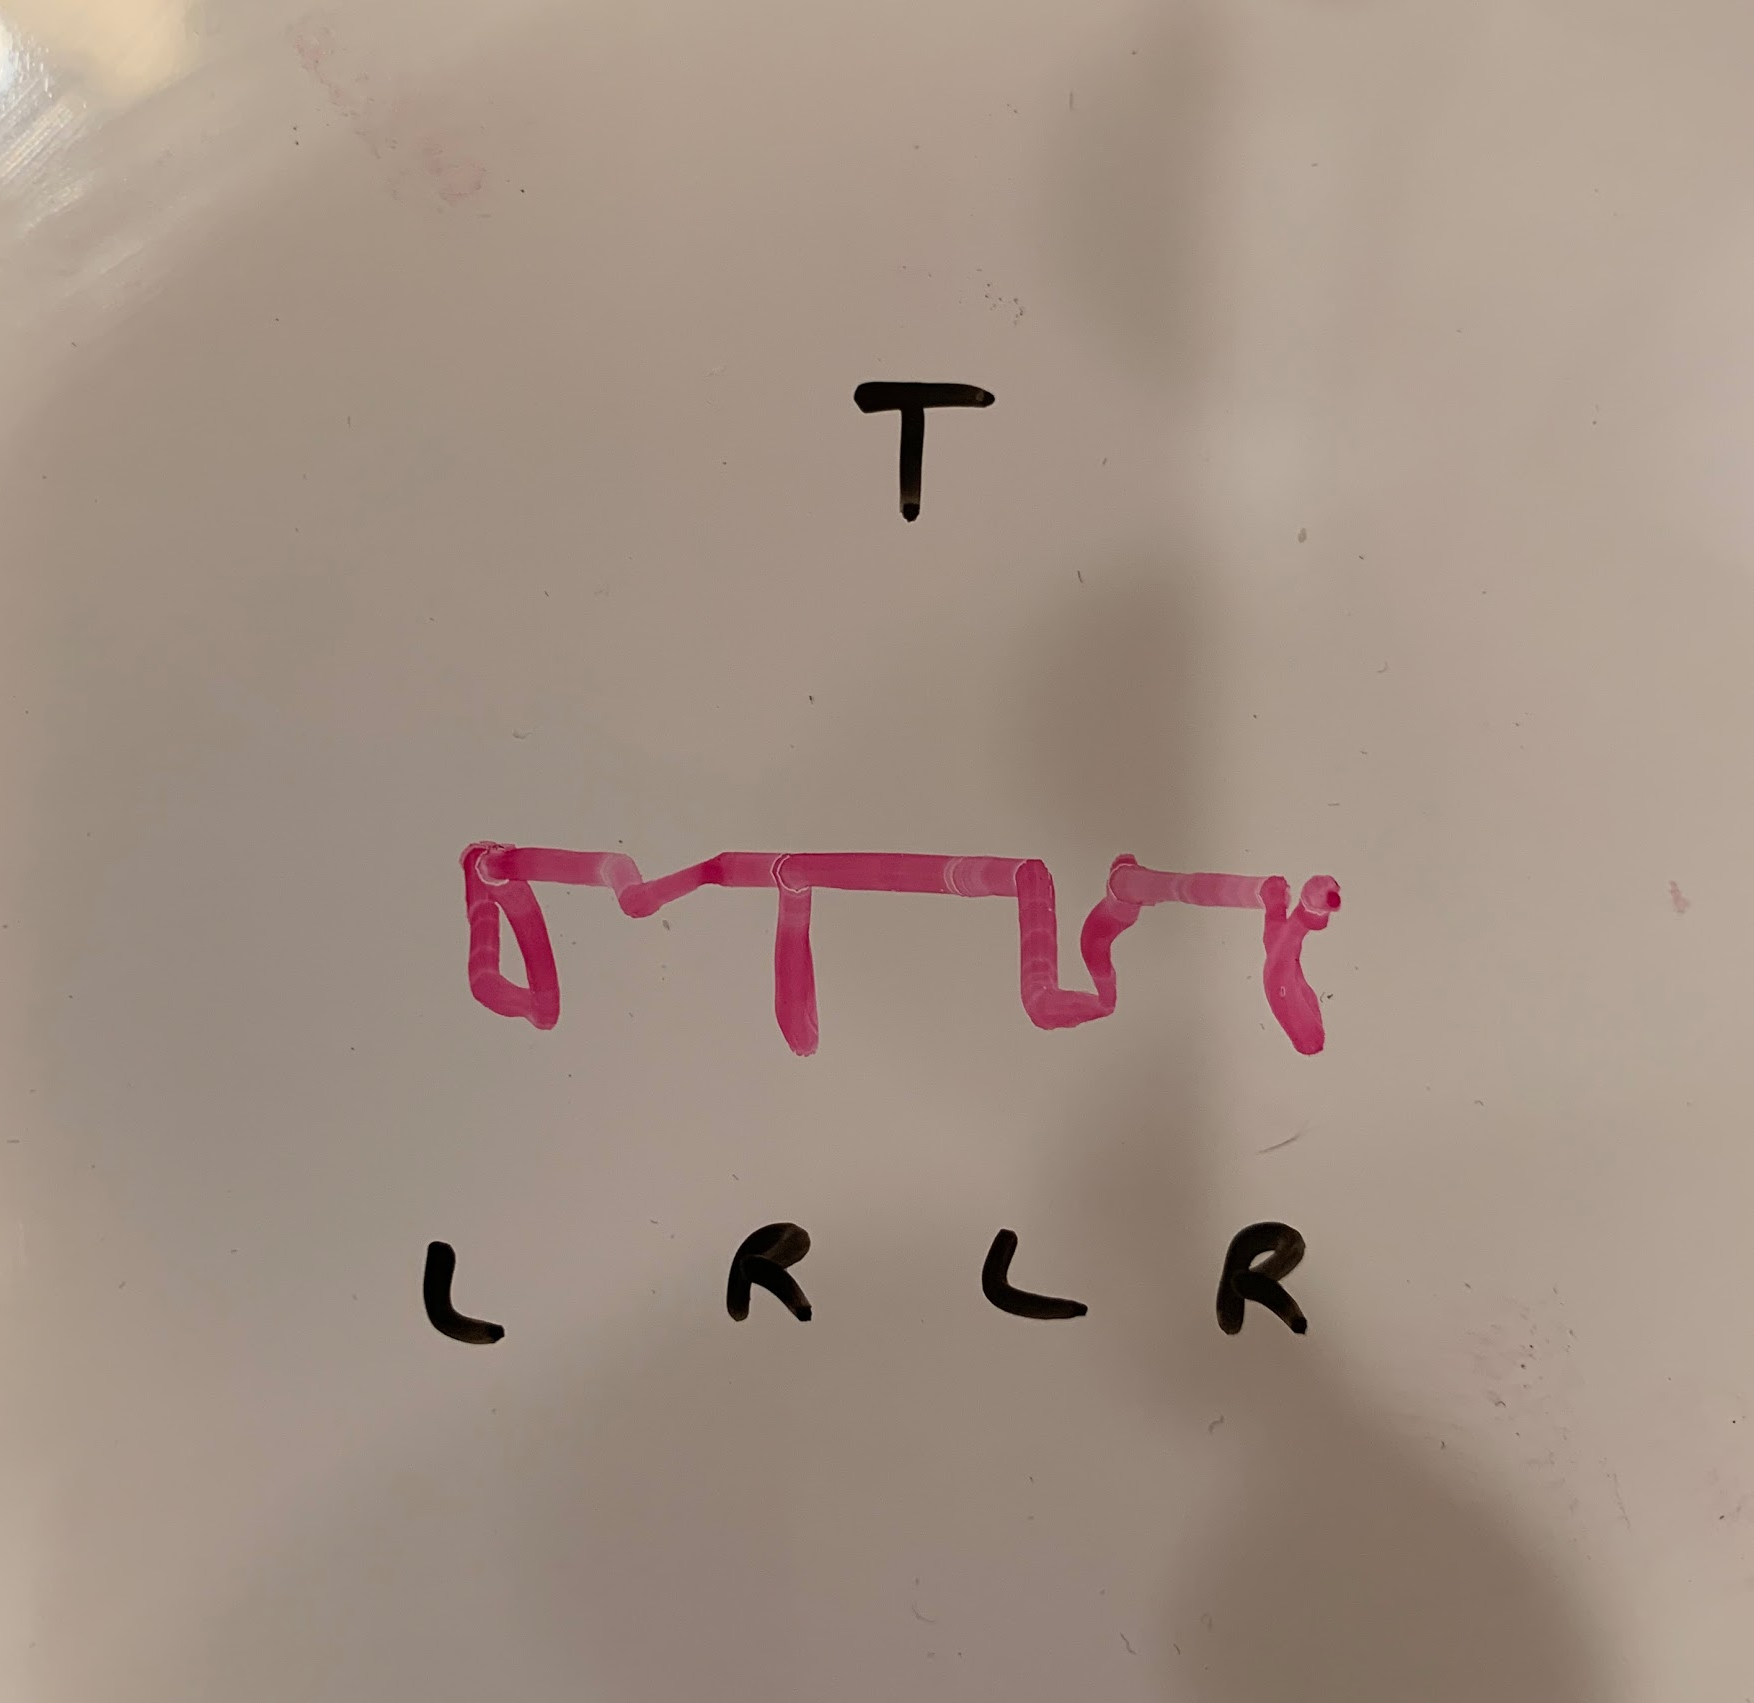
\includegraphics[width=0.29\columnwidth]{figures/results5.png}
\end{center}
\caption{Improvised force plate recordings of vertical ground reaction force; (a) and (b) trials comparing heel strike and toe strike; (c) checking toe strike. \textbf{Crop, fix annotate.}}
\label{fig:results:forceplate}
\end{figure}





\subsection{Measurements of acceleration using a smartphone}
\SI{10}{\second} recordings of the vertical ($Y$) acceleration during running with heel- and toe-strike are shown in~\fref{fig:results:accel}. Toe-strike appears to provide slightly higher peaks accelerations, but is not statistically different from heel-strike (ANOVA, $p=0.551$, $n=1998$). Vertical accelerations (mean$\pm$s.d.) are \SI{9.5\pm8.8} for heel-strike and \SI{9.3\pm10} for toe-strike. 
\begin{figure}
\begin{center}
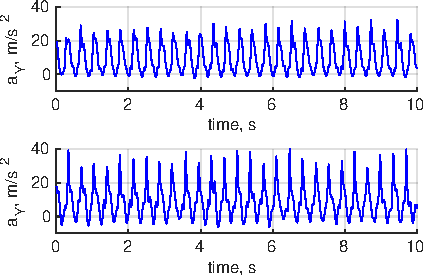
\includegraphics{data/accel/accelerations-raw.pdf}
\end{center}
\caption{$Y$ accelerations (approximately vertical) recorded during running with (a) heel-strike and (b) toe-strike. \textbf{Add A B annotations}}
\label{fig:results:accel}
\end{figure}





\subsection{Video kinematics on a treadmill}
\begin{figure}
\begin{center}
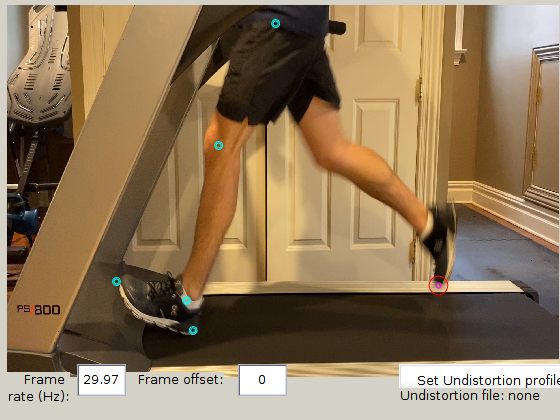
\includegraphics[width=0.29\columnwidth]{figures/point-references.png}
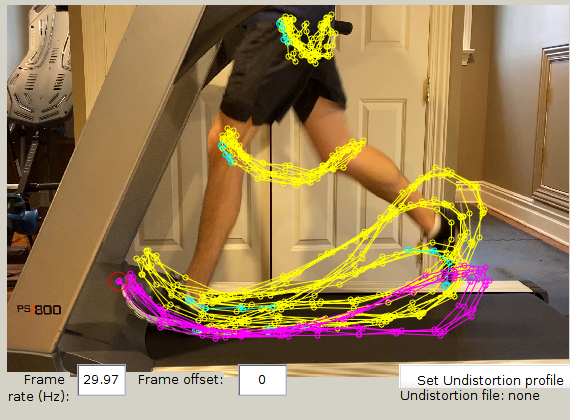
\includegraphics[width=0.29\columnwidth]{figures/heel-screenshot.png}
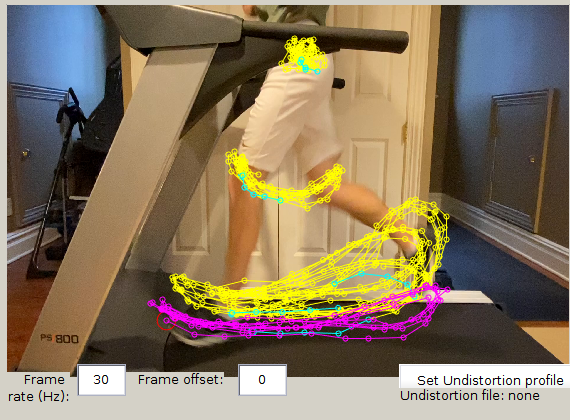
\includegraphics[width=0.29\columnwidth]{figures/toe-screenshot.png}
\end{center}
\caption{Digitzation points and example digitized points in (b) heel-strike and (c) toe-strike running, from dltdv8 \citep{hedrick2008software}. \textbf{Add annotations.}} 
\label{fig:methods:dltdv8-1}
\end{figure}


\begin{figure}
\begin{center}
% move these guys to methods?
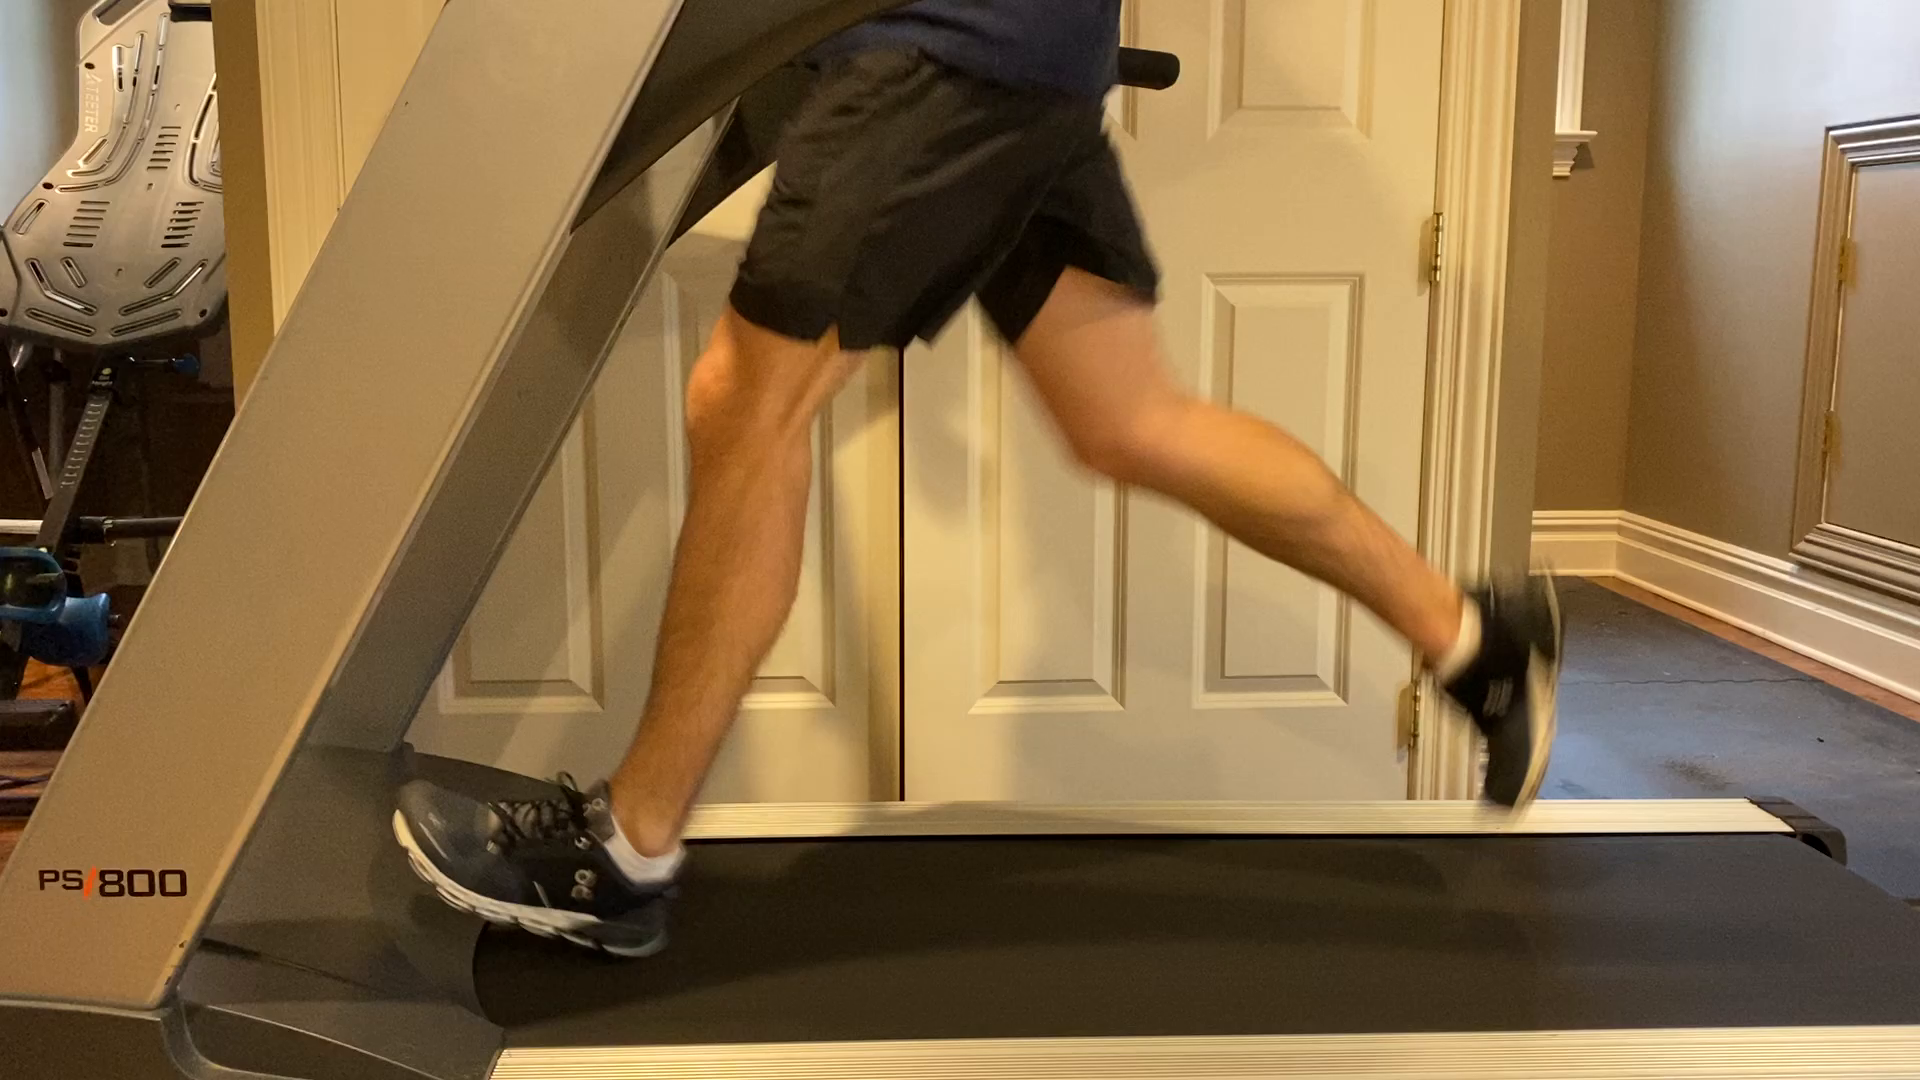
\includegraphics[width=0.29\columnwidth]{figures/heel_frames1.png}
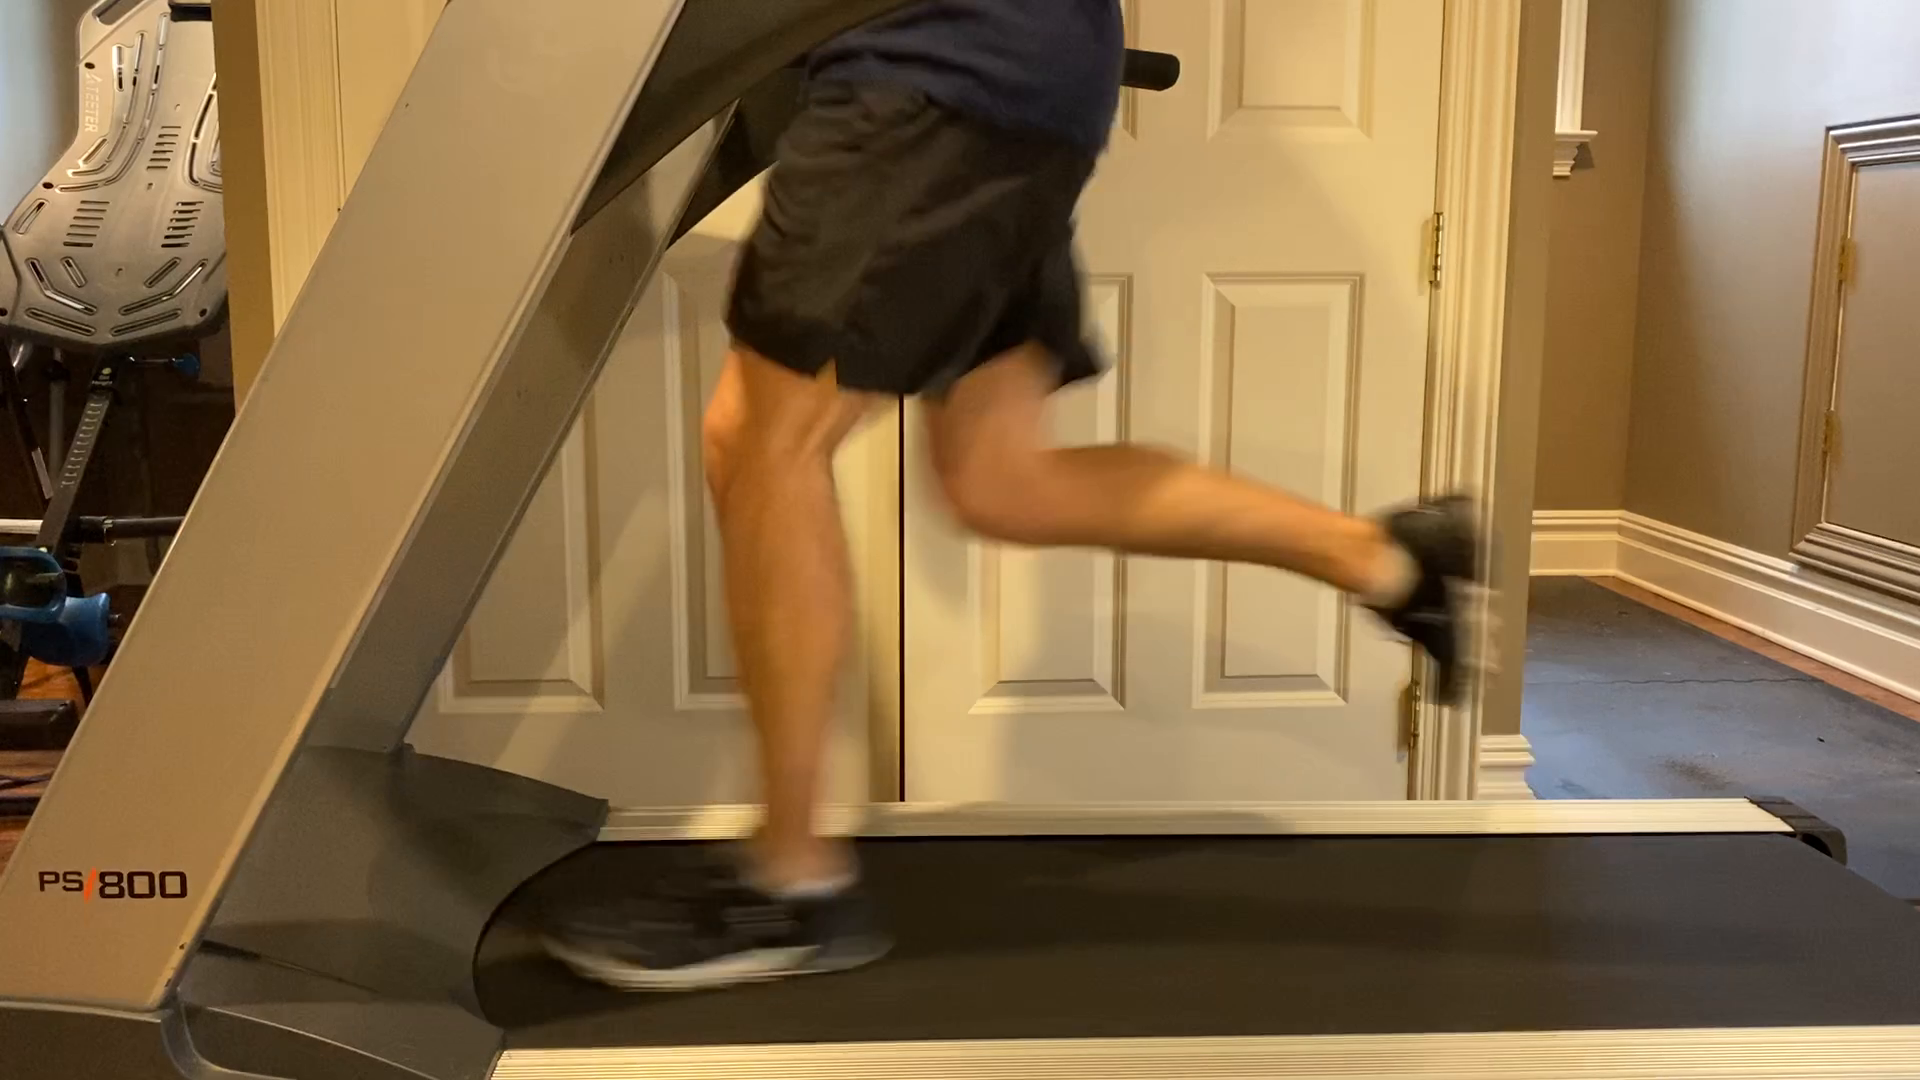
\includegraphics[width=0.29\columnwidth]{figures/heel_frames3.png}
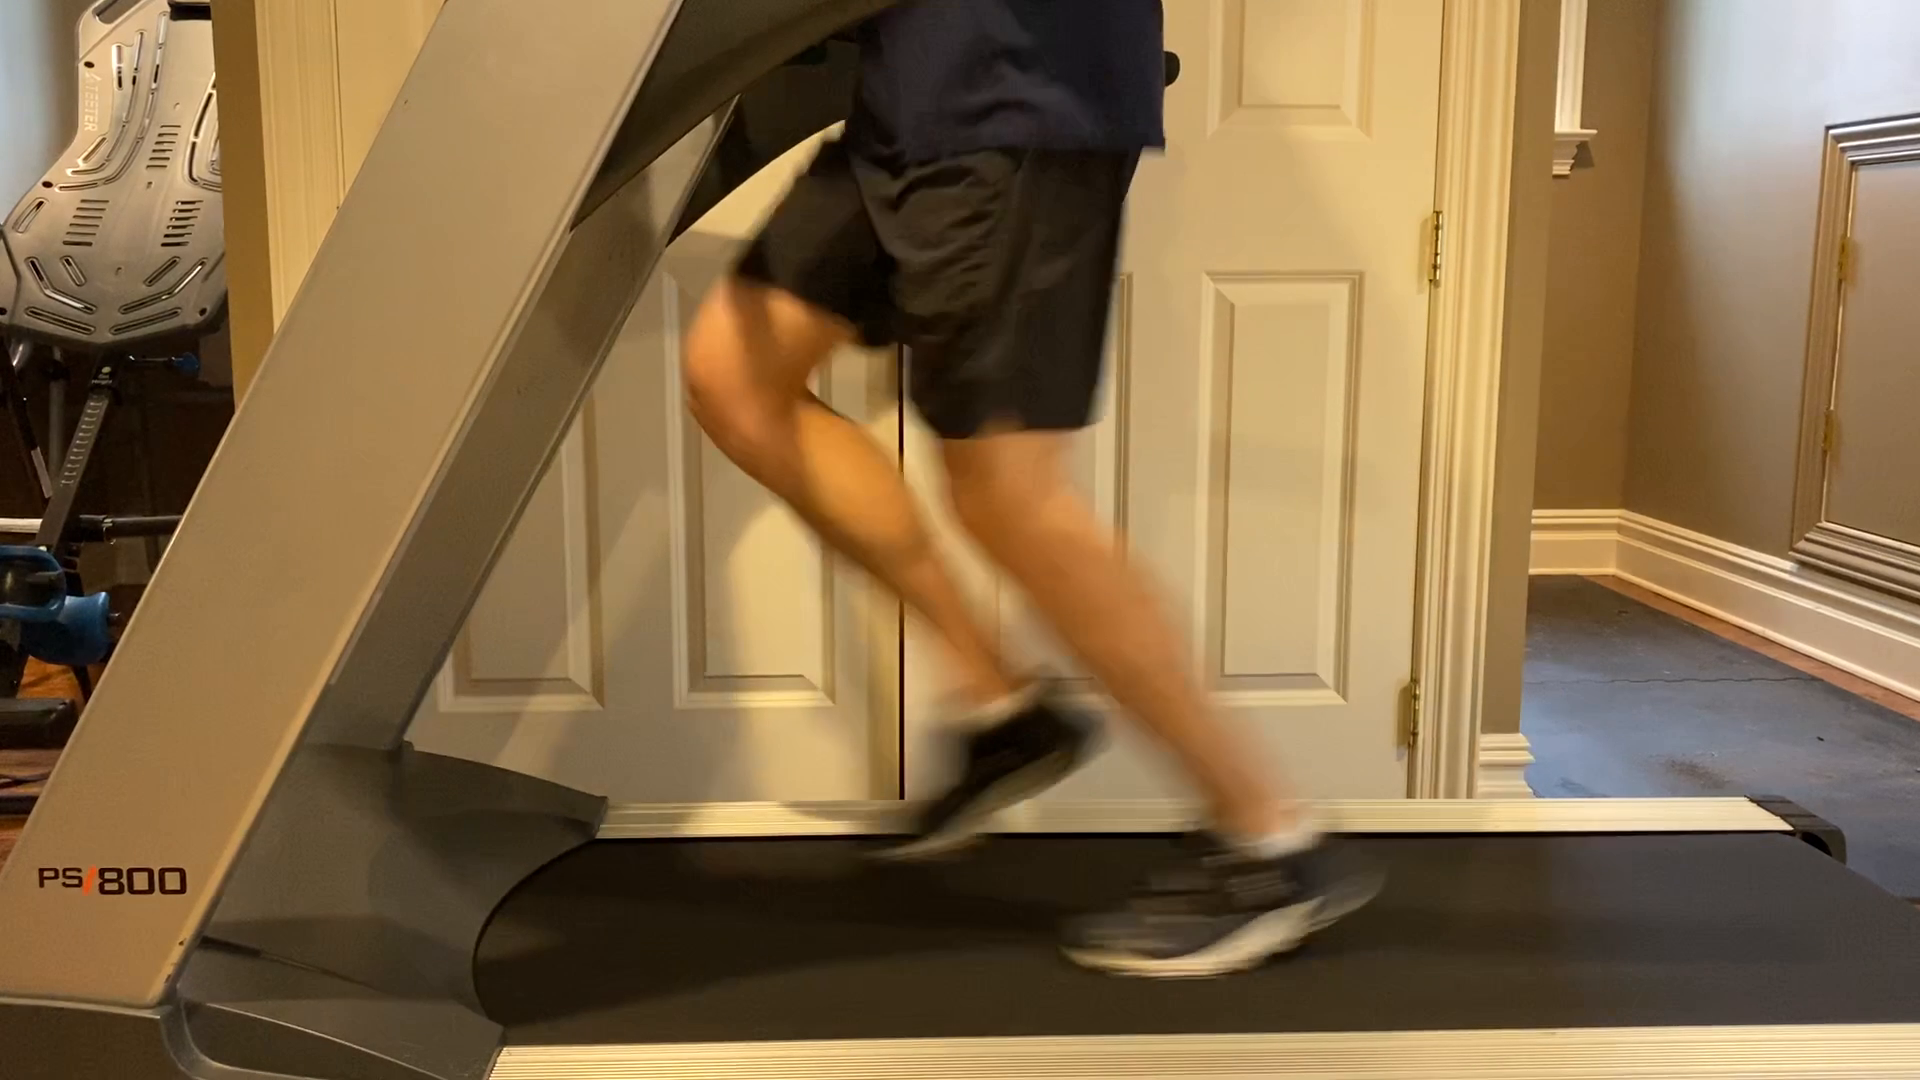
\includegraphics[width=0.29\columnwidth]{figures/heel_frames7.png}\\
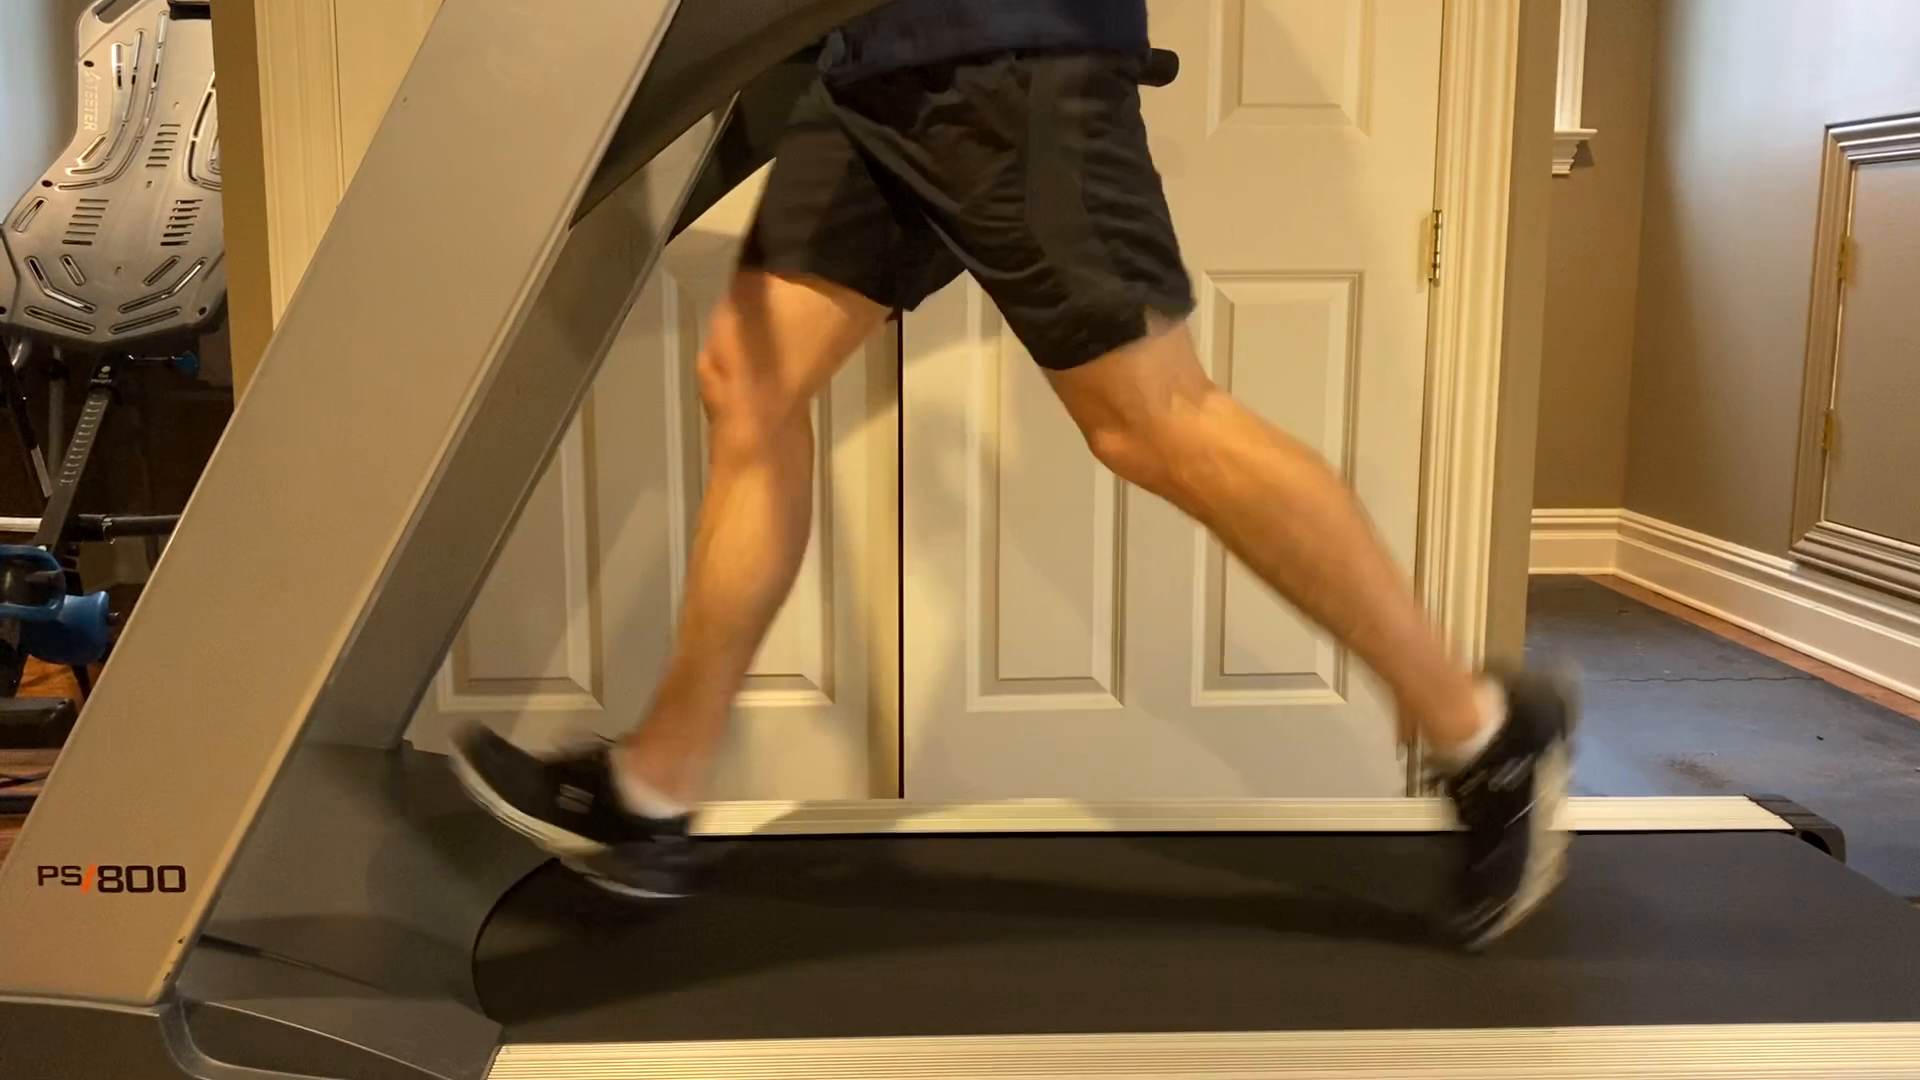
\includegraphics[width=0.29\columnwidth]{figures/heel_frames10.png}
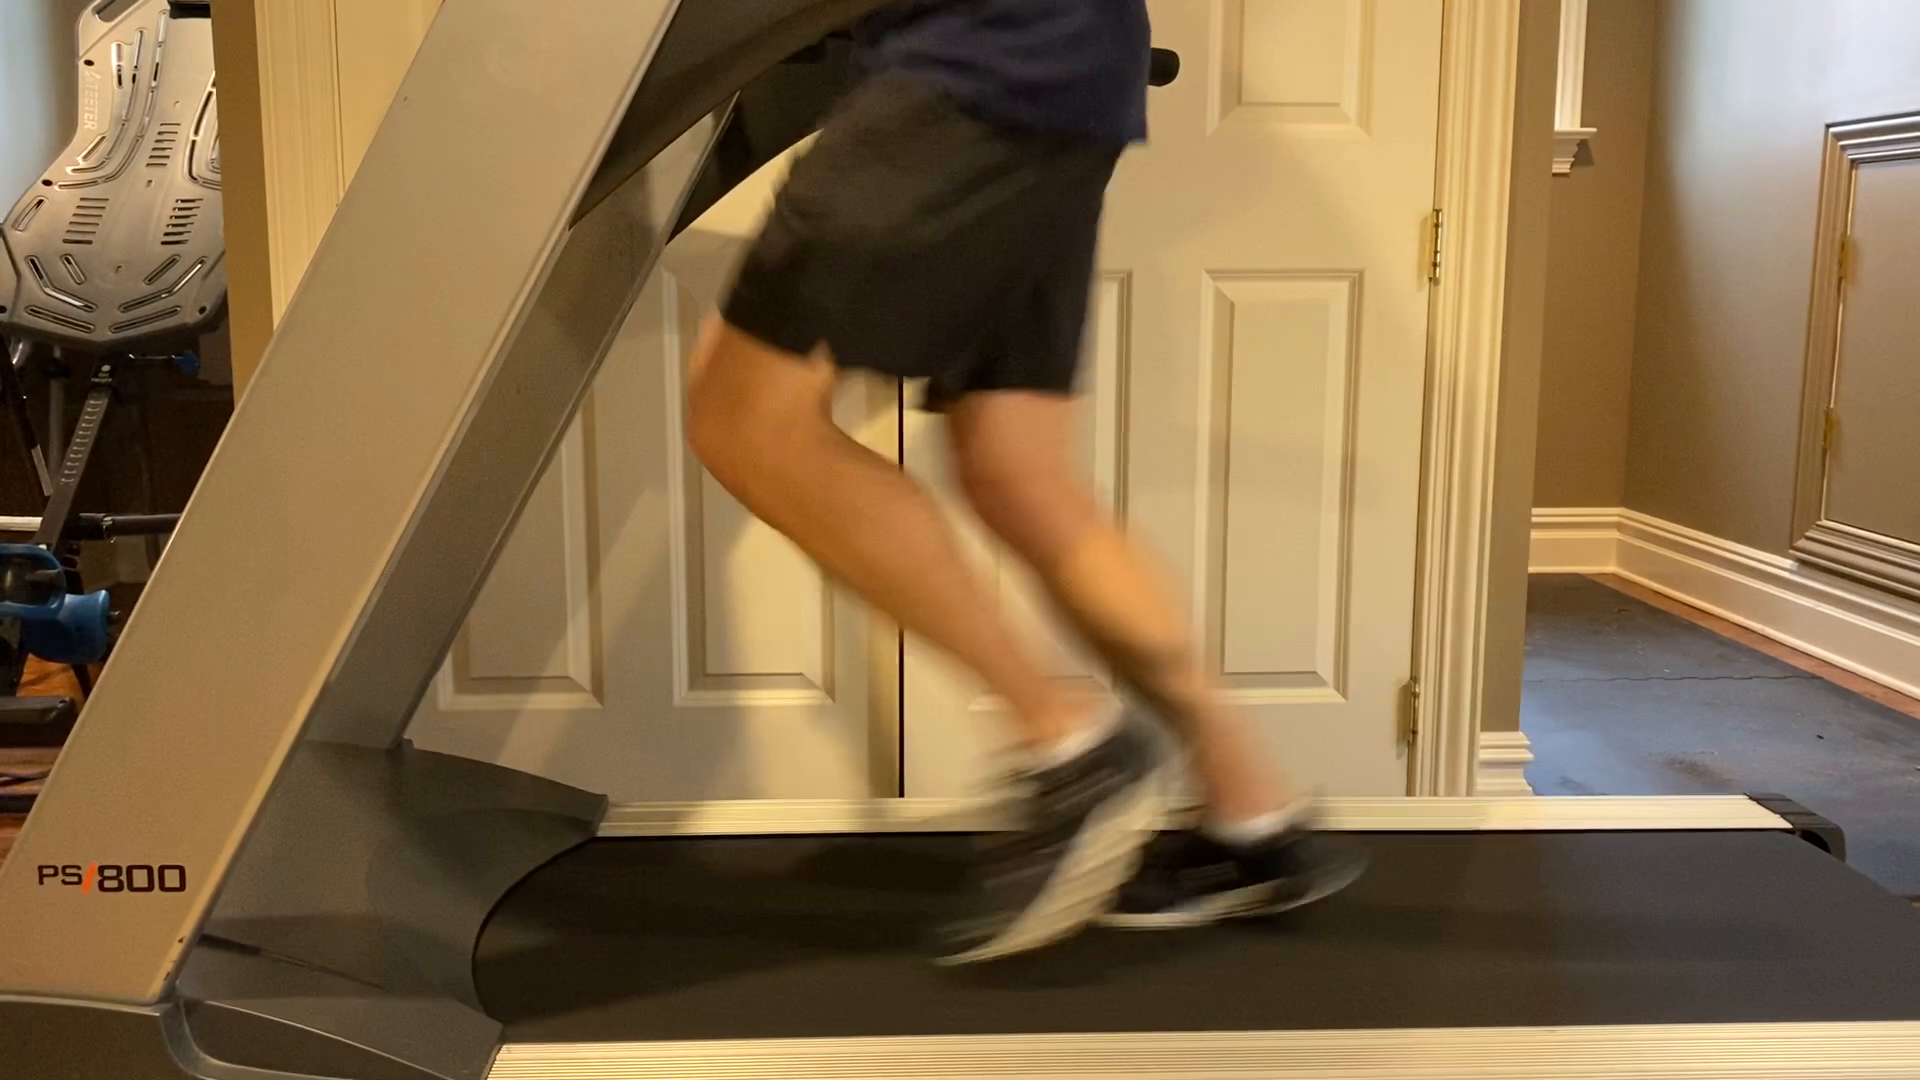
\includegraphics[width=0.29\columnwidth]{figures/heel_frames17.png}
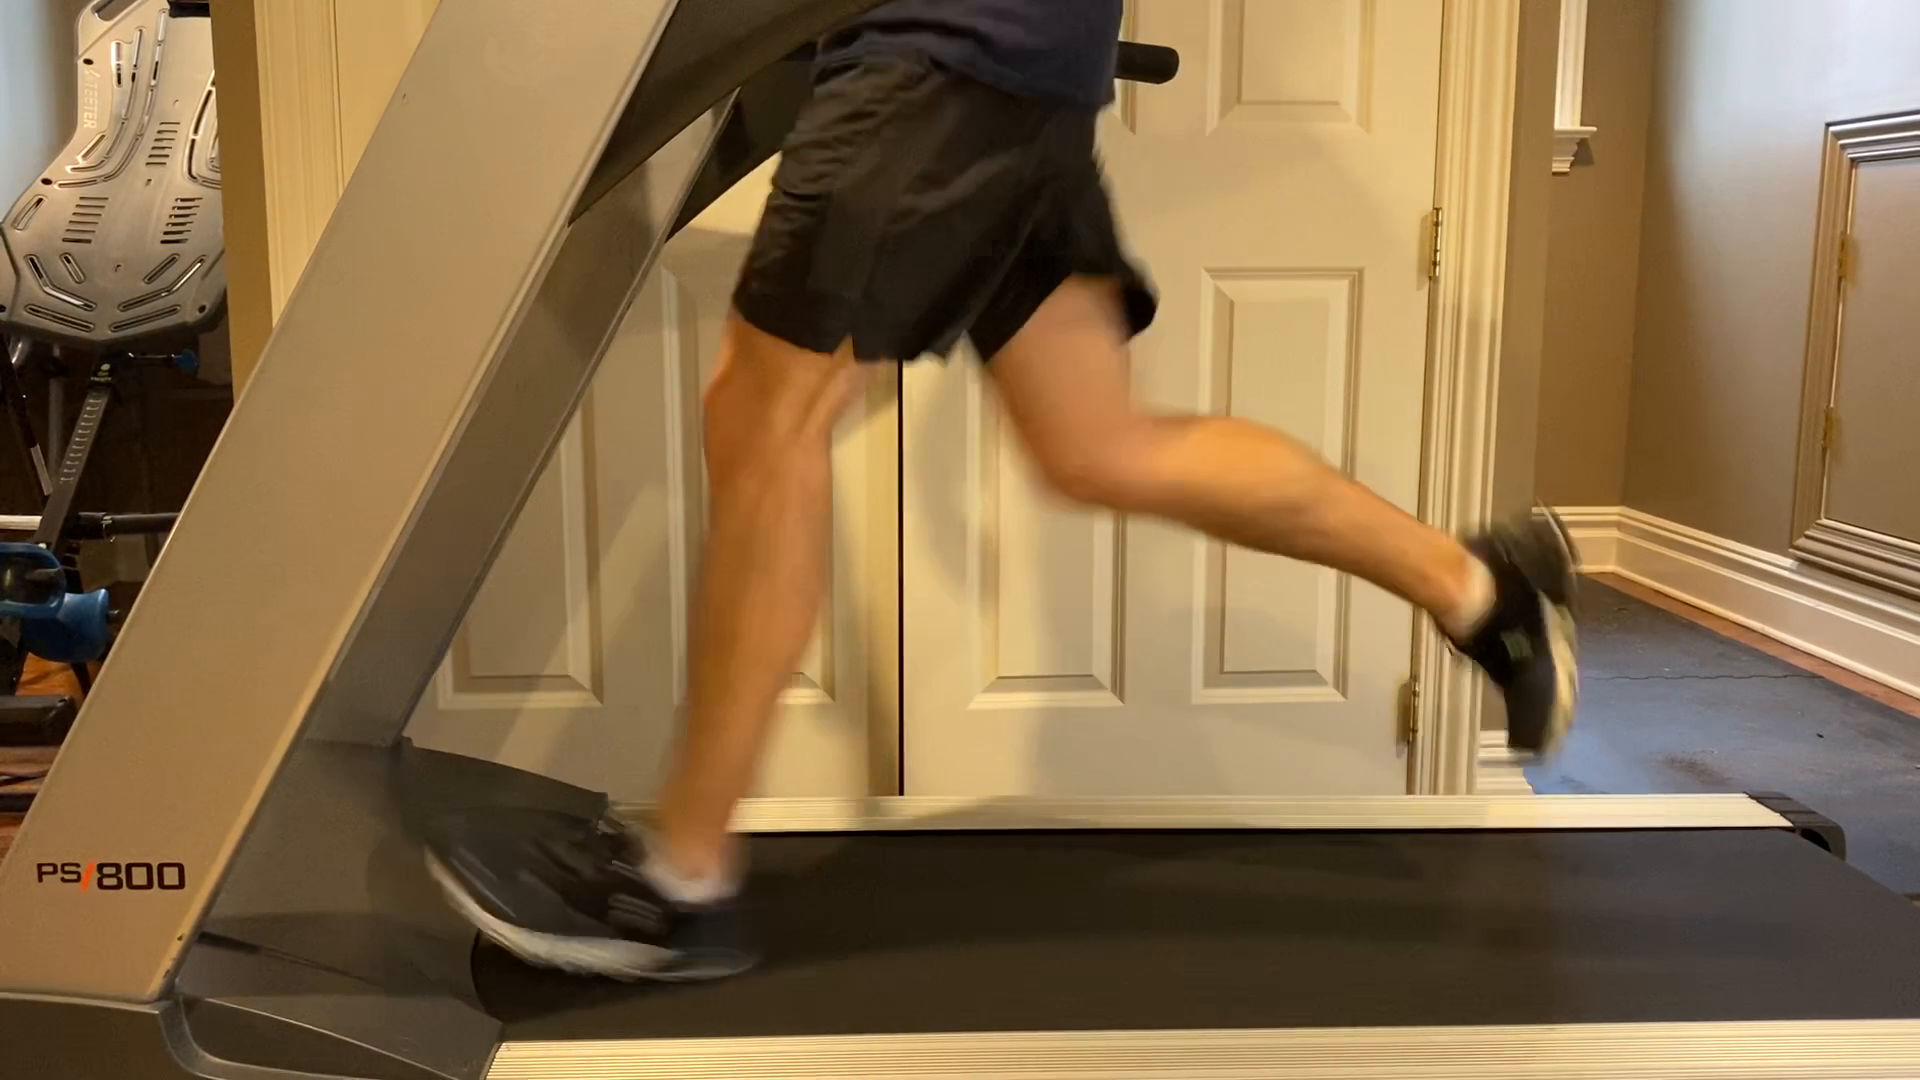
\includegraphics[width=0.29\columnwidth]{figures/heel_frames22.png}
\end{center}
\caption{Example video frames from running on a treadmill at \SI{8}{mph} (\SI{3.6}{\meter\per\second}), showing (a) heel-strike; (b) toe down; (d) toe up; and (f) start of the next step. \textbf{Add annotations.}} 
\label{fig:methods:dltdv8-2}
\end{figure}

\begin{figure}
\begin{center}
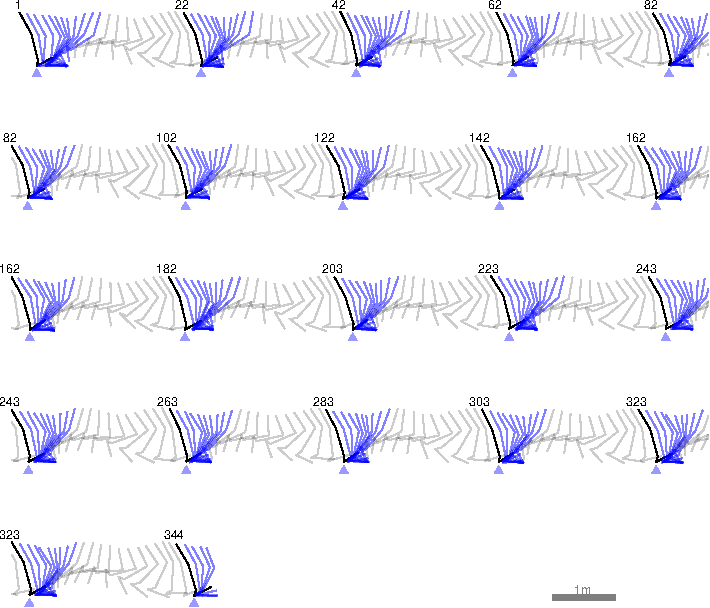
\includegraphics{data/heel-pretty.pdf}
\end{center}
\caption{Digitized kinematics from heel-strike running on a treadmill at \SI{8}{mph} (\SI{3.6}{\meter\per\second}). Heel strike position indicated with triangles. Stance phase for this leg indicated in blue. Numbers indicate video frame. Directions reversed from video. After \citep{marey1873locomotion, muybridge1901human}.}  
\label{fig:results:heelpretty}
\end{figure}

\begin{figure}
\begin{center}
\includegraphics{data/toe-pretty.pdf}
\end{center}
\caption{Digitized kinematics from toe-strike running on a treadmill at \SI{8}{mph} (\SI{3.6}{\meter\per\second}). Toe strike position indicated with triangles. Stance phase for this leg indicated in red. Numbers indicate video frame. Diretions reversed from video. After \citep{marey1873locomotion, muybridge1901human}.}  
\label{fig:results:toepretty}
\end{figure}

\begin{figure}
\begin{center}
\includegraphics{figures/stride-data.png}
\end{center}
\caption{Reduced stride data for 17 heel-strike and 21 toe-strike steps during running on a treadmill at \SI{8}{mph} (\SI{3.6}{\meter\per\second}), including (a) stride period; (b) stride frequency, (c) stride length and (d) duty cycle. Stastically significant differences marked; toe-strike stride period is shorter (ANOVA, $p=\num{4.7e-7}$, $n=17$), stride frequency is higher (ANOVA, $p=\num{5e-7}$), stride length is shorter (ANOVA, $p=\num{4.7e-7}$), and duty cycle is shorter (ANOVA, $p=\num{3e-10}$). See \fref{tab:results:stride}.} 
\label{fig:results:stride}
\end{figure}

\begin{table}
\caption{Reduced stride data (mean$\pm$s.d.) for 17 heel-strike and 21 toe-strike steps during running on a treadmill. Toe-strike stride period is shorter (ANOVA, $p=\num{4.7e-7}$, $n=17$), stride frequency is higher (ANOVA, $p=\num{5e-7}$), stride length is shorter (ANOVA, $p=\num{4.7e-7}$), and duty cycle is shorter (ANOVA, $p=\num{3e-10}$). See \fref{fig:results:stride}.}
\label{tab:results:stride}
\begin{center}
\begin{tabular}{lcc}
\toprule
& heel-strike ($n=17$) & toe-strike ($n=21$)\\
\midrule 
stride period, \si{\second}   & \num{0.67\pm0.01} & \num{0.64\pm0.02} \\
stride frequency, \si{\hertz} & \num{1.49\pm0.03} & \num{1.56\pm0.04} \\
stride length, \si{\meter}    & \num{2.41\pm0.05} & \num{2.29\pm0.06} \\
duty cycle                    & \num{0.46\pm0.03} & \num{0.40\pm0.02} \\
\bottomrule
\end{tabular}
\end{center}
\end{table}

\begin{figure}
\begin{center}
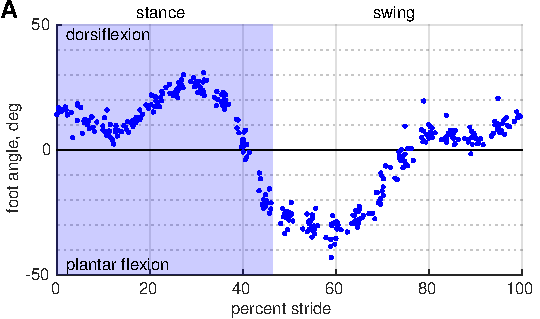
\includegraphics[width=0.49\columnwidth]{data/heel-foot-angle.pdf}
\includegraphics[width=0.49\columnwidth]{data/toe-foot-angle.pdf}\\
\includegraphics[width=0.49\columnwidth]{data/heel-knee-angle.pdf}
\includegraphics[width=0.49\columnwidth]{data/toe-knee-angle.pdf}\\
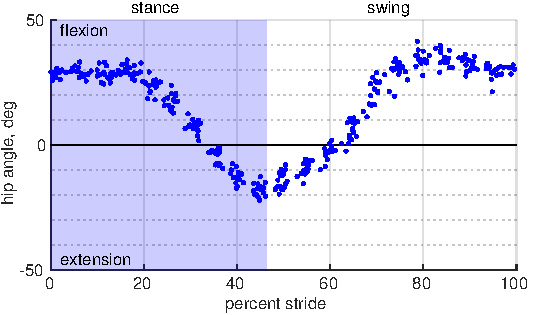
\includegraphics[width=0.49\columnwidth]{data/heel-hip-angle.pdf}
\includegraphics[width=0.49\columnwidth]{data/toe-hip-angle.pdf}
\end{center}
\caption{Joint angles for heel-strike and toe-strike running on a treadmill at \SI{8}{mph} (\SI{3.6}{\meter\per\second}). (a,b) Foot angle; (c,d) knee angle; (e,f) hip angle. Knee and hip angles appear similar between the two running styles, but foot angle shows clear differences immediately before and after foot contact with the ground. In heel-strike, the heel strikes with the foot dorsiflexed; while in toe-strike, the toe strikes the ground while the foot is plantar flexed, allowing it to act as a shock absorber. \textbf{Add annotations.}}
\label{fig:results:jointangles}
\end{figure}